\documentclass[tikz, border=10pt]{standalone}
\usetikzlibrary{arrows.meta, bending}

\begin{document}
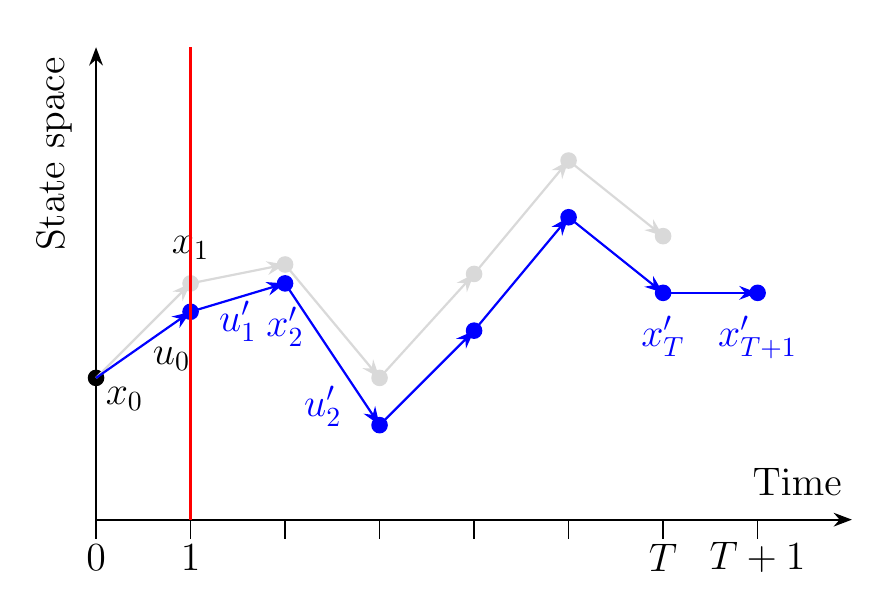
\begin{tikzpicture}[>=Stealth, scale=1.2]

    % Axes
    \draw[->, thick] (0,0) -- (8,0) node[anchor=south east, yshift=5pt] {\Large Time};
    \draw[->, thick] (0,0) -- (0,5) node[rotate=90, anchor=south east, yshift=5pt] {\Large State space};

    % Tick marks on x-axis
    \foreach \x in {0, 1, 2, 3, 4, 5, 6, 7}
        \draw (\x, 0) -- (\x, -0.2);
    
    % Axis labels
    \node at (0, -0.4) {\Large $0$};
    \node at (1, -0.4) {\Large $1$};
    \node at (6, -0.4) {\Large $T$};
    \node at (7, -0.4) {\Large $T+1$};

    % Define the points for the trajectory
    \coordinate (p0) at (0, 1.5);
    \coordinate (p1) at (1, 2.5);
    \coordinate (p2) at (2, 2.7);
    \coordinate (p3) at (3, 1.5);
    \coordinate (p4) at (4, 2.6);
    \coordinate (p5) at (5, 3.8);
    \coordinate (p6) at (6, 3);

    % Draw the smooth trajectory curve
    %\draw[ultra thick] (p0) to[out=30, in=180] (p1) 
    %                      to[out=0, in=170] (p2) 
    %                      to[out=-60, in=150] (p3) 
    %                      to[out=-30, in=210] (p4) 
    %                      to[out=30, in=160] (p5) 
    %                      to[out=-20, in=150] (p6);

    % Draw the nodes (dots)
    \foreach \p in {p0}
        \fill (\p) circle (2.5pt);

    \foreach \p in {p1, p2, p3, p4, p5, p6}
        \fill[gray!30] (\p) circle (2.5pt);

    
    % State Labels (x_k)
    \node[anchor=north west] at (p0) {\Large $x_0$};
    \node[anchor=south, yshift=5pt] at (p1) {\Large $x_1$};
    
    % Control Vectors (arrows u_k)
    \draw[->, thick, gray!30] (p0) -- (p1);
    \node at (0.8, 1.7) {\Large $u_0$};
    
    \draw[->, thick, gray!30] (p1) -- (p2);
    \draw[->, thick, gray!30] (p2) -- (p3);
    \draw[->, thick, gray!30] (p3) -- (p4);
    \draw[->, thick, gray!30] (p4) -- (p5);
    \draw[->, thick, gray!30] (p5) -- (p6);
    
    \coordinate (np1) at (1, 2.2);
    \coordinate (np2) at (2, 2.5);
    \coordinate (np3) at (3, 1.0);
    \coordinate (np4) at (4, 2.0);
    \coordinate (np5) at (5, 3.2);
    \coordinate (np6) at (6, 2.4);
    \coordinate (np7) at (7, 2.4);

    \node[anchor=north, yshift=-5pt, blue] at (np2) {\Large $x'_2$};
    \node[anchor=north, yshift=-5pt, blue] at (np6) {\Large $x'_T$};
    \node[anchor=north, yshift=-5pt, blue] at (np7) {\Large $x'_{T+1}$};

    \foreach \p in {np1, np2, np3, np4, np5, np6, np7}
        \fill[blue] (\p) circle (2.5pt);

    \draw[->, thick, blue] (p0) -- (np1);
    \draw[->, thick, blue] (np1) -- (np2);
    \draw[->, thick, blue] (np2) -- (np3);
    \draw[->, thick, blue] (np3) -- (np4);
    \draw[->, thick, blue] (np4) -- (np5);
    \draw[->, thick, blue] (np5) -- (np6);
    \draw[->, thick, blue] (np6) -- (np7);

    \draw[-, thick, red] (1,0) -- (1,5) node[anchor=south east]{};    

    \node[blue] at (1.5, 2.1) {\Large $u'_1$};
    \node[blue] at (2.4, 1.2) {\Large $u'_2$};

\end{tikzpicture}
\end{document}